\documentclass{beamer}

\usepackage{epstopdf}
\usepackage{float}
\usepackage{multicol}
\usepackage{booktabs}
\usepackage{chngpage}
\usepackage{IEEEtrantools,latexsym,amssymb,amsmath,mathrsfs}

\usetheme{Data61}

\title[CP applied to the MSPSP]{Constraint Programming applied to the Multi-Skill Project Scheduling Problem}
\author{Kenneth D. Young, Thibaut Feydy and Andreas Schutt}
\date{CP2017, 31st of August 2017}
% \institute, \subtitle are not implemented yet

\begin{document}

\maketitle
% alternatively use \frame[plain]{\titlepage}
% \frame{\tableofcontents}

\section{Introduction}
\subsection{Problem Definition}
\begin{frame}{Intro: The Problem}
	What is the Multi-Skill Project Scheduling Problem (MSPSP)?\pause
	\begin{itemize}
		\item Activites
		\item Workers
		\item Skills\pause
	\end{itemize}
	\vspace{4mm}
	\alert{Aim:} Find the fastest way to complete all the activities\pause\\
	\vspace{4mm}
	Constraints
	\begin{itemize}
		\item Activity constraint: Precedence relations between activities
		\item Skill constraint: Activities require skills
		\item Worker constraint: Workers each have a variety of skills
	\end{itemize}
\end{frame}

\subsection{Example}
\begin{frame}{Intro: Example}
	\scriptsize
	\begin{multicols}{2}
		\begin{table}
			\caption{Workers' Skills}
			\vspace{-3mm}
			\begin{tabular}{ccccc}
				\toprule
				 & Alice & Bob & Carl & Dora \\\midrule
				{\tiny {\bf Programmer}} & - & \checkmark & \checkmark & \checkmark \\
				{\tiny {\bf DB Designer}} & \checkmark & - & - & - \\
				{\tiny {\bf Webmaster}} & \checkmark & \checkmark & - & \checkmark \\
				\bottomrule
			\end{tabular}
		\end{table}\pause
		\begin{figure}[H]
			\includegraphics[width=\linewidth]{images/precgraph.eps}
			\caption{Precedence Graph}
		\end{figure}\pause
		\columnbreak

		\begin{table}
			\caption{Skill Requirement}
			\begin{tabular}{ccccc}
				\toprule
				 & $A_1$ & $A_2$ & $A_3$ & $A_4$ \\\midrule
				{\tiny {\bf Programmer}} & - & 1 & 2 & 1 \\
				{\tiny {\bf DB Designer}} & 1 & - & - & 1 \\
				{\tiny {\bf Webmaster}} & 1 & 1 & - & - \\
				\bottomrule
			\end{tabular}
		\end{table}\pause
		\vspace{-8mm}
		\begin{figure}[H]
			\includegraphics[width=\linewidth]{images/sched.eps}
			\caption{Schedule}
		\end{figure}

	\end{multicols}
\end{frame}

% \subsection{Constraint Programming}
% \begin{frame}{Intro: Constraint Programming}
% 	Domain propagation
% 	\begin{itemize}
% 		\item Variables have domains of possible values
% 		\item Constraints reduce the size of these domains
% 	\end{itemize}\pause
% 	Nogood learning
% 	\begin{itemize}
% 		\item Learn from failures
% 		\item Record these failures as constraints
% 		\item Use these constraints to make inferences
% 	\end{itemize}
% \end{frame}

\subsection{Previous Work}
\begin{frame}{Intro: The Literature}
	\begin{itemize}
		\item French research group
		\begin{itemize}
			\item Principal researchers: Odile Belleguez-Morineau, Emmanuel N\'{e}ron, Carlos Montoya
			\item Exact branch and bound methods
			\item Lower bounds
			\item Adapted data from PSPLib\pause
		\end{itemize}	
		\vspace{2mm}
		\item Portuguese research group
		\begin{itemize}
			\item Principal researchers: Bernardo Almeida, Isabel Correia, Francisco Saldanha-da-Gama
			\item Constructive heuristics
			\item Randomised search heuristics
			\item Generated their own data\pause
		\end{itemize}
		\vspace{2mm}
		\item Polish research group
		\begin{itemize}
			\item Principal researchers: Myszkowski, Skowronski
			\item Randomised search heuristics
			\item Generated their own data
		\end{itemize}
	\end{itemize}
\end{frame}

\begin{frame}{Intro: Timeline of the Literature}
	\begin{itemize}
		\item \color{red}{French} 
		\item \color{blue}{Portuguese} 
		\item \color{green}{Polish} 
		\item \color{darkgray}{Other} 
	\end{itemize}
	\begin{figure}[H]
		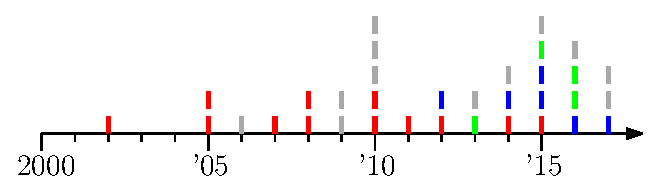
\includegraphics[width=0.8\linewidth]{images/lit_timeline.eps}
	\end{figure}
\end{frame}


%~~~~~~~~~~~~~~~~~~~~~~~~~~~~~~~~~~~~~~~~~~~~~~~~~~~~~~~~~~~~~~~~~~~~~~~~~~~~~~~~~%
% MODEL
\section{Model}
\subsection{Overview}
\begin{frame}{Model: Overview}
	\begin{itemize}
		\item \pause Objective
		\begin{itemize}
			\item Minimise the total project duration\pause
		\end{itemize}
	\end{itemize}
	\vspace{5mm}
	\begin{itemize}
		\item Two main decisions\pause
		\vspace{2mm}
		\begin{enumerate}
			\item Scheduling decisions
			\begin{itemize}
				\item Activity start times\pause
			\end{itemize}
			\vspace{2mm}
			\item Assignment decisions
			\begin{itemize}
				\item Workers to activities
				\vspace{1mm}
				\item Skill contribution of workers
			\end{itemize}
		\end{enumerate}
	\end{itemize}
\end{frame}

\subsection{Constraints}
\begin{frame}{Model: Constraints}
	\begin{itemize}
		\item \pause Precedence relations are respected\pause
		\vspace{2mm}
		\item Workers perform only one activity at a time\pause
		\vspace{2mm}
		\item Workers cannot multi-task\pause
		\vspace{2mm}
		\item Skill requirement is satisfied
		\begin{itemize}
			\item A worker for each skill must be present to perform the activity\pause
		\end{itemize}
		\vspace{2mm}
		\item Redundant constraints
	\end{itemize}
\end{frame}

\begin{frame}{Model: Choice of Constraints}
	Unary Resource Constraint
	\vspace{1mm}
	\begin{itemize}
		\item Each worker only performs one activity at a time\pause
	\end{itemize}
	\vspace{5mm}
	Possible ways of modelling\pause
	\vspace{1mm}
	\begin{enumerate}
		\item Time-indexed decomposition\pause
		\vspace{1mm}
		\item Global constraints (either disjunctive or cumulative)\pause
		\vspace{1mm}
		\item Order constraints
	\end{enumerate}
\end{frame}

\begin{frame}{Model: Decision Variables}
	\begin{adjustwidth}{-.9in}{-.9in}
	\begin{table}[h]
		\centering
		\vspace{1mm}
		\begin{tabular}{llp{8cm}}
			\toprule
			\multicolumn{3}{l}{ \bf{Decision Variables}}  \\
			\midrule
			Primary & $s_i$ & Start time of activity $i \in V$ \\
			 & $y_{ir}^s$ & 1 iff resource $r \in R$ contributes with skill $s \in S$ to activity $i \in V$\\\midrule
			% \multicolumn{2}{l}{\rule{0pt}{2ex} \bf{Auxilliary Decision Variables}}  \\
			Auxiliary & $o_{ij}$ & 1 iff activities $i$ and $j$ overlap for $(i,j)\in U$ \\
			 & $x_{ir}$ & 1 iff resource $r \in R$ is assigned activity $i \in V$ \\
			\bottomrule
		\end{tabular}
		\label{tab:vars}
	\end{table}
	\end{adjustwidth}
\end{frame}

\begin{frame}{Model}
	\begin{adjustwidth}{-.2in}{-.2in}
	\begin{IEEEeqnarray}{rClCl}
		\IEEEeqnarraymulticol{2}{r}{\text{Min}} & s_{n+1} & \hspace{4mm} & \label{objfun}\\
		\text{s.t. }\quad s_i + p_i &\leq& s_j & & \forall (i,j) \in E \label{const:prec}\\
		\neg o_{ij} &\Leftrightarrow& (s_i + p_i \leq s_j)\vee & & \nonumber\\
		\IEEEeqnarraymulticol{2}{r}{} & (s_j + p_j \leq s_i) & & \forall (i,j) \in U \label{const:unaryRes1}\\
		(x_{ir}\wedge x_{jr})&\Rightarrow& \neg o_{ij} & & \forall (i,j) \in U,~r \in RV_i \cap RV_j \label{const:unaryRes2}\\
		\sum_{r \in RV_i} y_{ir}^s&=& sr_{ik} \mathscr & & \forall i \in V,~s \in S_i \label{const:skillSatified}\\
		\sum_{s \in S_i | mast_{rk}=1} y_{ir}^s&\leq& 1 & & \forall i \in V,~r \in RV_i \label{const:noMultiTask}\\
		y_{ir}^s &\leq& mast_{rk} & & \forall i \in V,~r \in RV_i,~s \in S \label{const:mastery}\\
		y_{ir}^s &\leq& x_{ir} & & \forall i \in V, ~r \in RV_i, ~s \in S_i \label{const:linking}\\
		s_i &\geq& 0 & & \forall i \in V \label{const:nonfun1}
		% o_{ij},~x_{ir},~y_{irk} &\in&\IEEEeqnarraymulticol{3}{c}{\{0,1\} ~~ \forall (i,j) \in U, ~\forall i \in V~r \in \mathscr{R},~\forall i \in V~r \in \mathscr{R}~k \in \mathscr{L} \text{ resp.} } \label{const:nonfun2}
	\end{IEEEeqnarray}
	\end{adjustwidth}
\end{frame}

\begin{frame}{Model: Redundent Constraints}
	\begin{adjustwidth}{-.2in}{-.2in}
	\begin{IEEEeqnarray}{CCl}
		\IEEEeqnarraymulticol{1}{c}{{\tt cumulative}(s,~p,~[~sr_{ik}: i \in V],~|\mathscr{R}_k|)} & & \forall k \in \mathscr{L} \label{const:cumulSkill}\\
		\IEEEeqnarraymulticol{1}{c}{{\tt cumulative}\left(s,~p,~\left[~\sum_{k \in \mathscr{L}} sr_{ik}: i \in V~\right],~m\right)} & & \label{const:cumulRes}\\
		\IEEEeqnarraymulticol{3}{c}{x_{ir} = 0 ~~\forall i \in V,~r \in \mathscr{R}\backslash \mathscr{R}V_i} \label{const:redunAssign}\\
		\IEEEeqnarraymulticol{3}{c}{y_{irk} = 0 ~~\forall i \in V,~r \in \mathscr{R}\backslash \mathscr{R}V_i ,~k \in \mathscr{L}} \label{const:redunContribRes}\\
		\IEEEeqnarraymulticol{3}{c}{y_{irk} = 0 ~~\forall i \in V,~r \in \mathscr{R} ,~k \in \mathscr{L}\backslash \mathscr{L}_i} \label{const:redunContribSkill}\\
		\IEEEeqnarraymulticol{3}{c}{y_{irk} = 0 ~~\forall r \in \mathscr{R},~k \in \mathscr{L}\backslash \mathscr{L}_r,~i \in V} \label{const:redunContribAct}
	\end{IEEEeqnarray}
	\end{adjustwidth}
\end{frame}


%~~~~~~~~~~~~~~~~~~~~~~~~~~~~~~~~~~~~~~~~~~~~~~~~~~~~~~~~~~~~~~~~~~~~~~~~~~~~~~~~~%
% DATA
\section{Data}
\begin{frame}{Data: Overview}
	\begin{itemize}
		% \pause
		\item Tested on data from the literature and generated our own data\pause
	\end{itemize}
\begin{table}[tpb]
	\begin{adjustwidth}{-0.5cm}{}
    \setlength{\tabcolsep}{3pt}
    \centering
    \small
	\caption{Data sets summary}
	\begin{tabular}{@{}lrrrrrrr@{}}
		\toprule
		&  &  &  &  & \multicolumn{3}{c}{Best known results}\\ 
        \cmidrule(l){6-8} 
		set & \multicolumn{1}{l}{\#instances} & $n$ & $l$ & $m$ & source & \multicolumn{1}{r}{\%optimal} & {\color{red} \#unsolved} \\ \midrule
		1a     & 216 & 22 & 4 & 10-30 & Correia et al. 2012 & 93.98 & {\color{red} 13}\\
		1b     & 216& 42 & 4 & 20-60 & Almeida et al. 2016 & 2.31 & {\color{red} 211} \\ \midrule
		2a     & 110 & 20-51 & 2-8 & 5-14 & Montoya et al. 2014 & 43.64 & {\color{red} 62} \\
		2b     & 77 & 32-62 & 9-15 & 5-19 & Montoya et al. 2014 & 66.20 & {\color{red} 24} \\
		2c     & 91 & 22-32 & 3-12 & 4-15 & Montoya et al. 2014 & 51.11 & {\color{red} 44} \\ \bottomrule
	\end{tabular}
    \end{adjustwidth}
	\label{tab:data}
\end{table}
		% \begin{itemize}
		% 	\item equivalent to the Portuguese group's data\pause
		% \end{itemize}
	% 	\vspace{2mm}
	% 	\item Small data set: 216 unique instances
	% 	\begin{itemize}
	% 		\item 20 activities
	% 		\vspace{1mm}
	% 		\item 4 skills
	% 		\vspace{1mm}
	% 		\item 10-30 workers\pause
	% 		\vspace{1mm}
	% 		\item \alert{13 unsolved}\pause
	% 	\end{itemize}
	% 	\vspace{2mm}
	% 	\item Large data set: 216 unique instances
	% 	\begin{itemize}
	% 		\item 40 activities
	% 		\vspace{1mm}
	% 		\item 4 skills
	% 		\vspace{1mm}
	% 		\item 20-60 workers\pause
	% 		\vspace{1mm}
	% 		\item \alert{211 unsolved}
	% 	\end{itemize}
\end{frame}

\begin{frame}{Data: Complexity Measures}
	\begin{enumerate}
		\item Skill Factor
		\vspace{1mm}
		\begin{itemize}
			\item $SF \in \{1,~0.75,~0.5,~variable\}$\pause
		\end{itemize}
		\vspace{2mm}
		\item Network Complexity
		\vspace{1mm}
		\begin{itemize}
			\item $NC \in \{1.5,~1.8,~2.1\}$\pause
		\end{itemize}
		\vspace{2mm}
		\item Modified Resource Strength
		\vspace{1mm}
		\begin{itemize}
			\item varied over 3 values
			\item \[MRS=\frac{m}{\sum_{i\in V}\sum_{k \in \mathscr{L}}Req_{ik}}\]
		\end{itemize}
	\end{enumerate}
	% \vspace{3mm}
	% Therefore, 36 types of instances 
\end{frame}


%~~~~~~~~~~~~~~~~~~~~~~~~~~~~~~~~~~~~~~~~~~~~~~~~~~~~~~~~~~~~~~~~~~~~~~~~~~~~~~~~~%
% EXPERIMENTS
\section{Experiments}
% \subsection{Choosing Parameters}
% \begin{frame}{Experiments: Constraint Choice}
% 	Sample of 72 small instances\pause
% 	\begin{figure}[H]
% 		\includegraphics[width=0.8\linewidth]{images/constChoice.pdf}
% 	\end{figure}
% \end{frame}

\subsection{Results}
\begin{frame}{Experiments: Search Strategies}
	\begin{itemize}
		\item \pause Start times ($s_i$)
		\vspace{2mm}
		\item \pause Start times ($s_i$), then worker assignment ($x_{ir}$)
		\vspace{2mm}
		\item \pause Start times ($s_i$), then contrbution of each worker ($y_{irk}$)
		\vspace{2mm}
		\item \pause Na\"{i}ve priority search
	\end{itemize}
\end{frame}

\begin{frame}{Experiments: Small Data Set}
	\begin{itemize}
		\item Tested on all 216 small instances
		\item Time limit of 300 seconds \pause
	\end{itemize}
	\begin{table}[H]
		\begin{adjustwidth}{-.9in}{-.9in}
		\centering
		\scriptsize
		\begin{tabular}{r|rrrrrr}
			\hline
			search strategy & \#no soln & \%gap & \#optimal & \%optimal & avg. runtime  \\
			\hline
			default & 0 & 0.00 & 216 & 100.00 & 3.25s \\
			start &  0 & 2.50 & 215 & 99.54 & 1.26s \\
			start then worker & 0 & 0.00 & 216 & 100.00 & 2.89s \\
			\bf{start then skill} & \bf{0} & \bf{0.00} & \bf{216} & \bf{100.00} & \bf{1.63s} \\
			na\"{i}ve activity-based & 0 & 2.50 & 215 & 99.54 & 0.82s\\\pause
			activity smallest & 0 & 0.00 & 216 & 100.00 & 0.45s\\\hline
		\end{tabular}
		\end{adjustwidth}
	\end{table}
\end{frame}

\begin{frame}{Experiments: Large Data Set}
	\begin{itemize}
		\item Tested on all 216 large instances
		\item Time limit of 300 seconds \pause
	\end{itemize}
	\begin{table}[H]
		\begin{adjustwidth}{-.9in}{-.9in}
		\centering
		\scriptsize
		\begin{tabular}{r|rrrrrrrrr}
			\hline
			variable selection & \#nodes & \#props & \#no soln & \%gap & \#opt & \%opt & opt rt. & total rt.   \\
			\hline
			naive & 6,568k & 375m & 0 & 60.36 & 13 & 6.02 & 98.15 & 287.85 \\
			\bf{smallest} & \bf{734k} & \bf{71m} & \bf{0} & \bf{53.29} & \bf{15} & \bf{6.94} & \bf{103.51} & \bf{286.35} \\
			smallest\_largest & 814k & 73m & 0 & 55.50 & 7 & 3.24 & 70.71 & 292.57 \\
			first\_fail & 1,037k & 80m & 0 & 67.48 & 8 & 3.70 & 113.33 & 293.09 \\\pause
			smallest wth UB & 715k & 69m & 5 & 54.18 & 16 & 7.41 & 78.88 & 283.62 \\\pause
			smallest (fixed) & 3,962k & 409m & 0 & 50.18 & 24 & 11.11 & 55.45 & 272.83 \\\hline
		\end{tabular}
		\end{adjustwidth}
	\end{table}
\end{frame}

\begin{frame}{Experiments: Large Data Set}
	\begin{itemize}
		\item Time limit of 3600 seconds \pause
	\end{itemize}
	\begin{table}[H]
		\begin{adjustwidth}{-.9in}{-.9in}
			\centering
			\scriptsize
			\vspace{2mm}
			\begin{tabular}{cc|rrrrrrrr}
				\hline
				measure & value  & \#nodes & \#props & \%gap & \#opt & \%opt & opt rt. &  total rt. \\
				\hline SF & 1 & 36m & 4,254m & 48.35 & 7 & 12.96 & 257.55 & 3166.72 \\
				 & 0.75 & 47m & 4,296m & 49.63 & 4 & 7.41 & 545.44 & 3373.74 \\
				 & 0.5 & 32m & 4,468m & 42.06 & 20 & 37.04 & 782.20 & 2556.37 \\
				 & var & 45m & 4,302m & 49.82 & 5 & 9.26 & 130.97 & 3278.79 \\\hline
				NC & 1.5 & 41m & 5,007m & 57.33 & 8 & 11.11 & 819.48 & 3291.05 \\
				 & 1.8 & 42m & 4,381m & 46.09 & 11 & 15.28 & 558.06 & 3135.26 \\
				 & 2.1 & 36m & 3,602m & 38.99 & 17 & 23.61 & 446.41 & 2855.40 \\\hline
				MRS & \#1 & 37m & 6,083m & 76.93 & 14 & 19.44 & 327.52 & 2963.68 \\
				 & \#2 & 42m & 4,154m & 43.36 & 8 & 11.11 & 913.89 & 3301.54 \\
				 & \#3 & 39m & 2,753m & 23.94 & 14 & 19.44 & 599.07 & 3016.49 \\\hline
				\hline \bf{Overall} &  & \bf{40m} & \bf{4,330m} & \bf{47.92} & \alert{\bf{36}} & \bf{16.67} & \bf{563.43} & \bf{3093.90} \\\hline\hline
			\end{tabular}
		\end{adjustwidth}
	\end{table}
\end{frame}

%~~~~~~~~~~~~~~~~~~~~~~~~~~~~~~~~~~~~~~~~~~~~~~~~~~~~~~~~~~~~~~~~~~~~~~~~~~~~~~~~~%
% CONCLUSION
\section{Conclusion}
\subsection{Summary}
\begin{frame}{Summary}
	\begin{itemize}
		\item Applied the constraint programming solver chuffed to the MSPSP\pause
		\vspace{2mm}
		\item Generated a set of benchmark instances\pause
		\vspace{2mm}
		\item Found an effective model formulation\pause
		\vspace{2mm}
		\item Solved all small instances
	\end{itemize}
\end{frame}

% \subsection{Future Work}
% \begin{frame}{Future Work}
% 	\begin{itemize}
% 		\item Apply activity-based search to the large dataset\pause
% 		\vspace{2mm}
% 		\item Create a more structured search procedure in chuffed
% 	\end{itemize}
% \end{frame}

\begin{frame}{Acknowledgements}
	\begin{itemize}
		\item Dr. Andreas Schutt
		\vspace{2mm}
		\item Dr. Thibaut Feydy
		\vspace{2mm}
		\item Adrian Goldwaser
	\end{itemize}
\end{frame}

\begin{frame}{}
	\centering
	{\Large Thanks for listening!\vspace{1cm}\\
	Questions?}
\end{frame}

\end{document}
